\documentclass[a4paper,12pt]{book}

% This package can be used to create margins
\usepackage[a4paper, inner=1.7cm, outer=2.7cm, top=2cm, bottom=2cm, bindingoffset=1.2cm]{geometry}

% This package can be used to add some random text
\usepackage{blindtext}

%Package to make lists look better
\usepackage{enumitem}

%package for better looking header
\usepackage{fancyhdr}

%Package for math formulae
\usepackage{amsmath}

%to auto generate index
\usepackage{index}
\makeindex %This generates the index

%To add pictures into the document
\usepackage{graphicx}

%We use this package for creating newline and linebreak
\usepackage[utf8]{inputenc}

%End of priamble

\begin{document} %Must be present in all LaTex Documents

\title{\Large{\textbf{Latex Learning}}}
\author{By Guru Sarath Thangamani}
\date{August 31st 2020}
\maketitle %This line creates the title page
\let\cleardoublepage\clearpage %This line is required to remove the blank page that gets created
\tableofcontents %This creates the content page

\pagenumbering{roman} %use roman numeral for page numbering
\setcounter{page}{2} %Start numbering from page 2

%
% Using the Fancy header package
%
\fancyhf{} %Clear default header and footer
\renewcommand{\headrulewidth}{2pt}
\renewcommand{\footrulewidth}{1pt}
\fancyhead[LE]{\leftmark} %LE - even page
\fancyhead[LE]{\nouppercase}{\leftmark} %RO odd page
\fancyfoot[LE,RO]{\thepage} %\thepage - show only page number

\chapter{Introduction}

\section{Text Section}
\blindtext[5] %Add some random text

\section{List Section}
%
% Creating a list
%
\setlist{nolistsep} %This maked the list more compact (removes the space between lines)

\textbf{Unordered List}
\begin{itemize}
	\item 1 Cup
	\item Banana
	\item Carrot
	\item Eating
	\begin{itemize}
		\item salt
		\item pepper
		\item Last item
	\end{itemize}
	\item new
\end{itemize}
\  \\ %This is the only way that I found to add a new line after a list
\textbf{Numbered List}
\begin{enumerate}[label=\Roman*, font=\bfseries]
	\item Testing some item
	\begin{itemize}
		\item salt
		\item pepper
		\item Last item
	\end{itemize}
	\item itemY
	\item itemZ
	\item itemX
\end{enumerate}
\  \\ 
\textbf{Description list}
\begin{description}
	\item[Current] Current is rate of flow of charges
	\item[Voltage] Thing that pushes the current
\end{description}

\section{New Random Section}
\blindmathtrue %Add some blind math formulae
\blindtext[5]
\pagebreak

\section{Figure Section}
\blindtext
%
% Adding a figure
%
\begin{figure}[ht] % h - here t - top;  There is also hb - here bottom
	\centering
	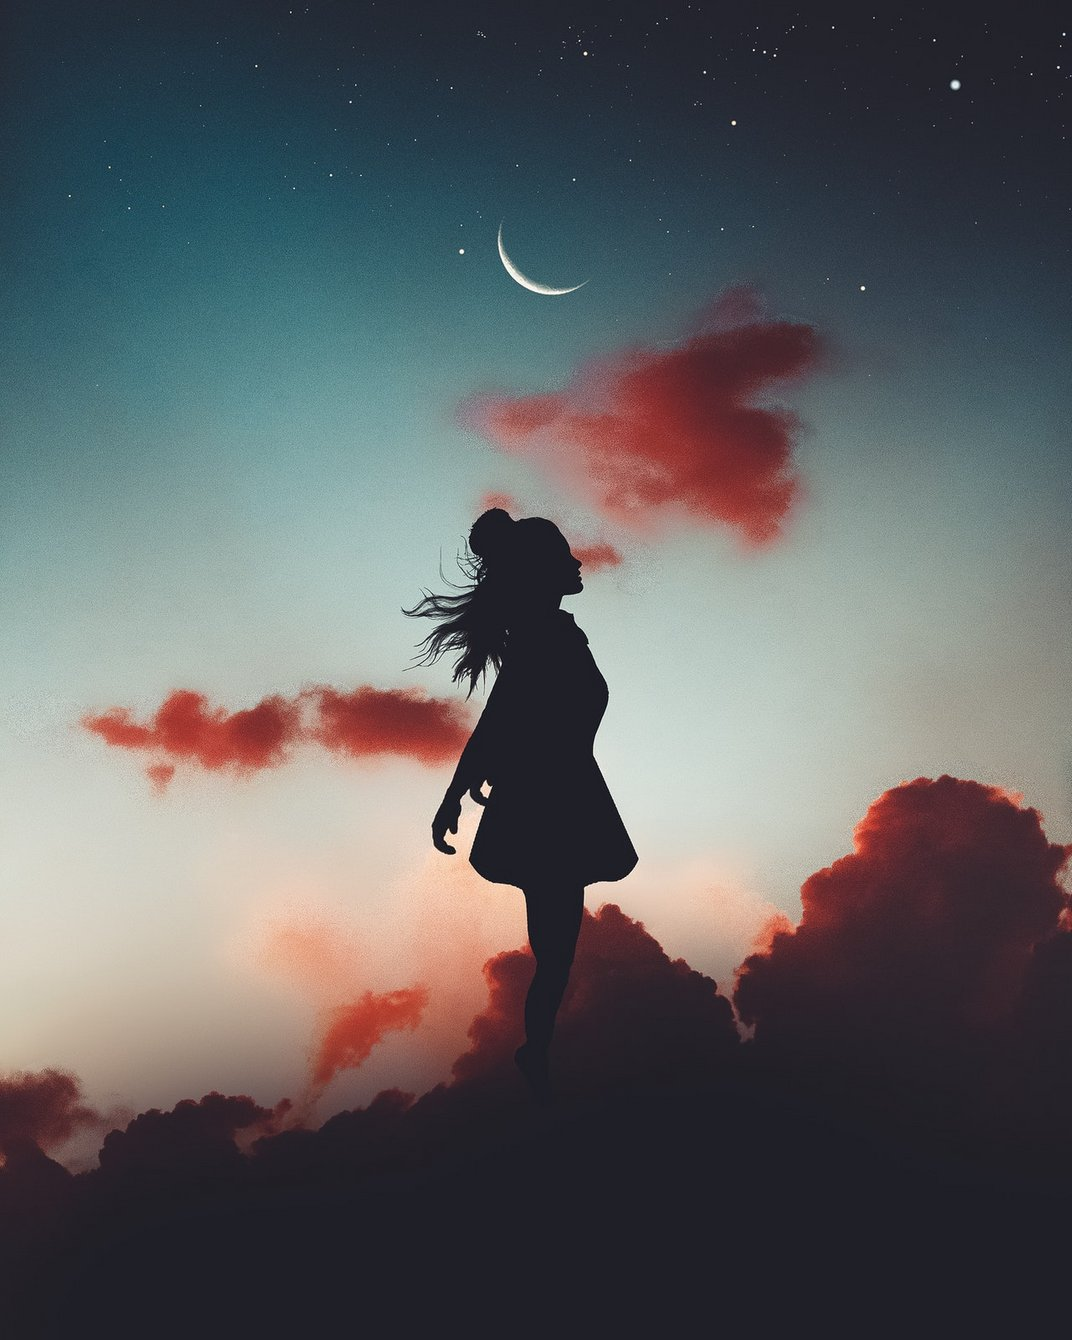
\includegraphics[width=8cm]{pic.jpg}
	\end{figure}
\blindtext

\section*{Section C.1 (This section will not be listed in the contents page)} %* indicates that the seciton will not be listed in the table of contents
\blindtext
\pagebreak

\section{Section Tabbing}
%
% Tabbing
%
\begin{tabbing}
	Customer \= Name \hspace*{1.5cm} \= Street \hspace*{1.5cm} \= City \\ %Heading
	\> Guru Sarath \> Lincoln \> Madurai \\ % \> Jumps to the next tab
	\> Priya \> Ball Street \> Dindigul \\
\end{tabbing}

\section{Section Table}
%
% Table
%
\begin{table}[ht]
	\centering
	\begin{tabular}{|c|c|c|} % c - center ( l - left, r - right ) ( | - draw vertical line)
		\hline %horizontal line
		\textbf{Name} & \textbf{Street} & \textbf{City}\\
		\hline
		Guru Sarath & Lincoln & College \\
		Priya & Ball Street & Madurai \\
		\hline
	\end{tabular}
	\caption{This is the caption of the table}
\end{table}

\section{Section Text emphasis}
%
% Text Emphasis and size
%
\emph{This is emph text}\\
\textit{This is textit text}\\
\textsc{This is textsc text}\\
\textmd{This is textmd text}\\
\textup{This is textup text}\\
\textrm{This is textrm text}\\
\textsf{This is textsf text}\\
\texttt{This is texttt text}\\
\textbf{This is textbf text}\\

\normalsize{normal size}\\
\small{small}\\
\scriptsize{scriptsize}\\
\tiny{tiny}\\
\large{large}\\
\Large{Large}\\
\LARGE{LARGE}\\
\huge{huge}\\
\Huge{Huge}\\

\begin{tiny}
This is inside the tiny block
\end{tiny}

\end{document} %Must be present in all LaTex Documents










